\documentclass{article}
%% Language and font encodings
\usepackage[english]{babel}
\usepackage[utf8x]{inputenc}
\usepackage[T1]{fontenc}

%% Sets page size and margins
\usepackage[a4paper,top=3cm,bottom=2cm,left=3cm,right=3cm,marginparwidth=1.75cm]{geometry}

%% Beautiful code writing
\usepackage{listings}

%% Beautiful citations
\usepackage{cite}

%% Let arrays of equations to happen without aligning 
\usepackage{array}

%% Allows subfigures 
\usepackage{subcaption}
\usepackage{caption}

%% Fix plots and tables
\usepackage{float}

%% Will make it easy to center, justify ... the text
\usepackage[document]{ragged2e}

%% Useful packages
\usepackage{amsmath}
\usepackage{graphicx}
\usepackage[colorinlistoftodos]{todonotes}
\usepackage[colorlinks=true, allcolors=blue]{hyperref}
\usepackage{bm}
\usepackage{tikz}
\usetikzlibrary{arrows}
\usepackage{xcolor}

%% Useful table package
\usepackage{tabularx}

%% Multiple columns
\usepackage{multicol}
%% For coding
\definecolor{gray97}{gray}{.97}
\definecolor{gray75}{gray}{.75}
\definecolor{gray45}{gray}{.45}

\definecolor{mygreen}{rgb}{0,0.6,0}
\definecolor{mygray}{rgb}{0.5,0.5,0.5}
\definecolor{mymauve}{rgb}{0.58,0,0.82}

\lstset{ frame=Ltb,
framerule=0pt,
aboveskip=0.5cm,
framextopmargin=3pt,
framexbottommargin=3pt,
framexleftmargin=0.4cm,
framesep=0pt,
rulesep=.4pt,
backgroundcolor=\color{gray97},
rulesepcolor=\color{black},
%
stringstyle=\ttfamily,
showstringspaces = false,
basicstyle=\small\ttfamily
commentstyle=\color{gray45},
keywordstyle=\bfseries,
%
numbers=left,
numbersep=15pt,
numberstyle=\tiny,
numberfirstline = false,
breaklines=true,
}

\lstdefinestyle{customc}{
  belowcaptionskip=1\baselineskip,
  breaklines=true,
  frame=XXL,
  xleftmargin=\parindent,
  language=C,
  showstringspaces=false,
  basicstyle=\footnotesize\ttfamily,
  keywordstyle=\bfseries\color{black},
  commentstyle=\itshape\color{mygray},
  identifierstyle=\color{blue},
  stringstyle=\color{mygreen},
}

\lstdefinestyle{custompy}{
  belowcaptionskip=1\baselineskip,
  breaklines=true,
  frame=XXL,
  xleftmargin=\parindent,
  language=Python,
  showstringspaces=false,
  basicstyle=\footnotesize\ttfamily,
  keywordstyle=\bfseries\color{black},
  commentstyle=\itshape\color{mygray},
  identifierstyle=\color{blue},
  stringstyle=\color{mygreen},
}

%% For algorithms
\usepackage{algorithm}
\usepackage[noend]{algpseudocode}

\definecolor{mycolor}{rgb}{0.822, 0.915, 0.898}% Rule colour


\begin{document}

\title{SF2568: Homework 2}
\date{\today}
\author{\begin{tabular}{l r}
      Daniel Persson Proos & dproos@kth.se \\
      Borja Rodríguez Gàlvez & borjarg@kth.se \\
    \end{tabular}}

\maketitle

\begin{enumerate}

\item 

\begin{enumerate}

\item In order to do a on-to-all broadcast we make use of the recursive doubling idea as you can see in Algorithm \ref{broadcast}.

There are small subtilities in the algorithm that do not appear in the standard all-to-all exange of information. Now we have a process, $SOURCE$, which sends the message to all the other processes; therefore, we have to ensure that at each step of the recusrive doubling only the processes which contain the message send it and the others receive it. In order to overcome this we first look at the case where the source is the process 0 and then we will be able to easiliy generalize to process $SOURCE$; where $SOURCE \in [0, P-1]$.

When the source process is 0 we can apply recursive doubling having only the processes where the first bit changes taking action (i.e., process 1 receiving and process 0 sending). After doing that, we can repeat this setting with the ones that change only the second bit; having the ones with null second bit sending and the active second bit receiving (i.e., 0 and 1 sending and 2 and 3 receiving). Then, we continue this setting until all processes have received the message. If the number of processes is not a power of 2 (i.e., $2^D < P < 2^{D+1}$) we only have to check if the process we have to send to exists or not, since the receiving process will have strictly a higher number than ours. An example of that is shown in Figure \ref{fig:broadcast_pic}.

\begin{figure}[H]
  		\centering
  		
  		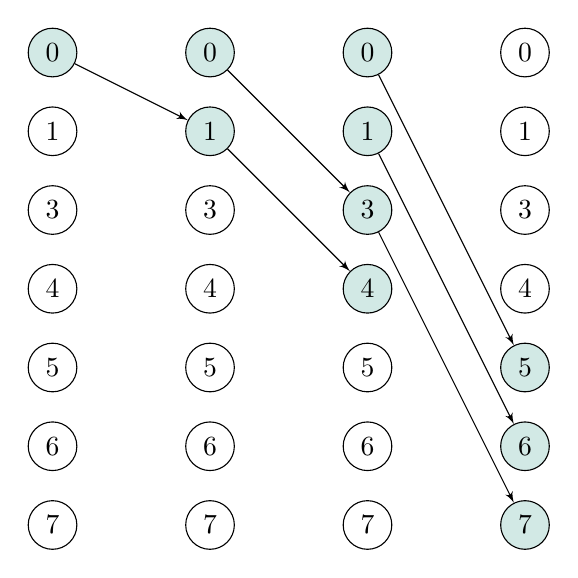
\begin{tikzpicture}

		\tikzset{vertex/.style = {shape=circle,draw,minimum size=1.5em}}
		\tikzset{edge/.style = {->,> = latex'}}
		% vertices
		% First nodes
		\node[vertex, fill = mycolor] (00) at (0,0) {0};
		\node[vertex] (10) at (0,-1) {1};
		\node[vertex] (20) at (0,-2) {3};
		\node[vertex] (30) at (0,-3) {4};
		\node[vertex] (40) at (0,-4) {5};
		\node[vertex] (50) at (0,-5) {6};
		\node[vertex] (60) at (0,-6) {7};
		% Second nodes
		\node[vertex, fill = mycolor] (01) at (2,0) {0};
		\node[vertex, fill = mycolor] (11) at (2,-1) {1};
		\node[vertex] (21) at (2,-2) {3};
		\node[vertex] (31) at (2,-3) {4};
		\node[vertex] (41) at (2,-4) {5};
		\node[vertex] (51) at (2,-5) {6};
		\node[vertex] (61) at (2,-6) {7};
		% Third nodes
		\node[vertex, fill = mycolor] (02) at (4,0) {0};
		\node[vertex, fill = mycolor] (12) at (4,-1) {1};
		\node[vertex, fill = mycolor] (22) at (4,-2) {3};
		\node[vertex, fill = mycolor] (32) at (4,-3) {4};
		\node[vertex] (42) at (4,-4) {5};
		\node[vertex] (52) at (4,-5) {6};
		\node[vertex] (62) at (4,-6) {7};
		% Forth nodes
		\node[vertex] (03) at (6,0) {0};
		\node[vertex] (13) at (6,-1) {1};
		\node[vertex] (23) at (6,-2) {3};
		\node[vertex] (33) at (6,-3) {4};
		\node[vertex, fill = mycolor] (43) at (6,-4) {5};
		\node[vertex, fill = mycolor] (53) at (6,-5) {6};
		\node[vertex, fill = mycolor] (63) at (6,-6) {7};
		
		%edges
		% First edges
		\draw[edge] (00) to (11);
		% Second edges
		\draw[edge] (01) to (22);
		\draw[edge] (11) to (32);
		% Third edges
		\draw[edge] (02) to (43);
		\draw[edge] (12) to (53);
		\draw[edge] (22) to (63);
	

		\end{tikzpicture}  	
			
  		\caption{Example of 0-source one-to-all broadcast with 7 processes.}
    	\label{fig:broadcast_pic}
\end{figure} 

When the source node is not 0, we can just create a maping to all the processes to another name (in the Algorithm \ref{broadcast} we call it $myRank$) in which the source is 0 and all the other processes have a unique identifier in the same range of values and (i.e., 0 to P-1). This way we use the same previous technique but looking at this new identifier instead of looking at the process rank. An easy bit-wise operation that does this job is an $XOR$ with the source rank.


\begin{algorithm}
\caption{Broadcast Algorithm}\label{broadcast}
\begin{algorithmic}[1]
\Procedure{broadcast(source, MESSAGE)}{}
\State // D is the bit length s.t. $2^D \leq P \leq 2^{D+1}$
\State mask = $2^{D+1} - 1$
\State // $rank$ is the process rank
\State // Change the rank values so $rank$ is equivalent to $0$ 
\State myRank = SOURCE XOR $rank$
\For{d = 0 $\rightarrow$ $D+1$}
	\State // Updating the mask for the bits we are considering
	\State mask = bitflip(mask, d)
	\State // Checking if our rank is being considered for sending or receiving
	\If{mask AND myRank = 0}
		\State q = bitflip(p,d)
		\State // We only continue if the process exists
		\If {q < P}
			\State // If the bit is off send else receive
			\If{myRank AND $2^d$ = 0}
				\State send(q, MESSAGE)
			\Else
				\State MESSAGE = receive(q)
			\EndIf	
		\Else
			\State break
		\EndIf
	\EndIf
\EndFor
\EndProcedure
\end{algorithmic}
\end{algorithm}

\item For the time analysis of the algorithm we define the following variables to be $t_{su}$: set up time; $t_d$: transfer data time; $t_a$: action time; and $m$: message length. With this definition the communication time is directly:

\begin{equation}
	t_{comm} = (D+1)(t_{su} + m t_d) \approx \log P (t_{su} + m t_d)
\end{equation}

Then, we can compute the computation time as follows:

\begin{equation}
	t_{comp} = 2 t_a + (D+1) (2 t_a + 3 t_a) \approx \log P (5 t_a),
\end{equation}

where the first $2 t_a$ account from the generation of the mask and the $XOR$ operation with the source; the first $2 t_a$ multiplying $(D+1)$ account for the two bitflips and the last $3 t_a$ multiplying $(D+1)$ come from the comparisons and $ANDs$. Therefore, the total time is approximately,

\begin{equation}
	t_P \approx \log P (t_su + m t_d + 5 t_a)
\end{equation}

which is indeed an $\mathcal{O}(\log P)$ algorithm.

\item The scatter algorithm (Algorithm \ref{scatter}) share the same ideas than the one-to-all broadcast algorithm. For this algorithm we are asked to spread the information on one processor among all the processors (see Figure \ref{fig:scatter} for an example).

In order to develop this algorithm it is enough to apply the same skeleton that the broadcasting algorithm had but now sending only halves of the message each time. The problem that arises doing this algorithm is only that the messages would not be ordered as they would be in a linear distribution fashion. To overcome this problem we can simply rearange the message puting the first half to be only the even positions of the message (i.e., 0, 2, 4, ...) and the last half to be the odd positions (i.e., 1, 3, 5 ...). This way we are following the mask order and they will be distributed as in a linear data distribution.

Again, this distribution is only linear if the source process is process 0. To overcome this, we can simply save the new id for each process (i.e., $myRank$) and the data will be linearly distributed over the process in these new process indexing.

As in the previous exercise, this algorithm is $\mathcal{O}(\log P)$, since no additional communications are done that they were not in the one-to-all broadcasting.

\begin{figure}[H]
\centering
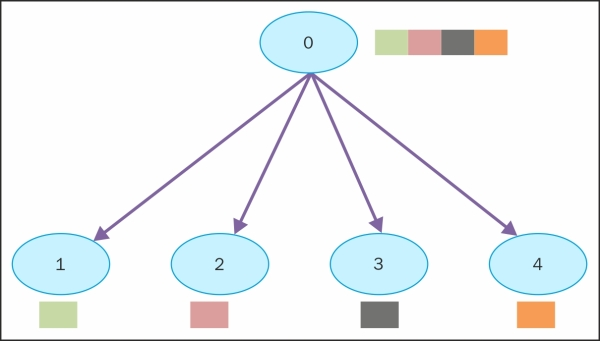
\includegraphics[scale=1.5]{scatter_ex.jpg}
\caption{Scatter operation with 0-source and linear data distribution with 4 processes.}
\label{fig:scatter}
\end{figure}

\begin{algorithm}
\caption{Scatter Algorithm}\label{scatter}
\begin{algorithmic}[1]
\Procedure{scatter(source, MESSAGE)}{}
\State // D is the bit length s.t. $2^D \leq P \leq 2^{D+1}$
\State mask = $2^{D+1} - 1$
\State // $rank$ is the process rank
\State // Change the rank values so $rank$ is equivalent to $0$ 
\State myRank = source XOR $rank$
\For{d = 0 $\rightarrow$ $D$}
	\State // Updating the mask for the bits we are considering
	\State mask = bitflip(mask, d)
	\State // Checking if our rank is being considered for sending or receiving
	\If{mask AND myRank = 0}
		\State q = bitflip(p,d)
		\State // We only continue if the process exists
		\If {q < P}
			\State // If the bit is off send else receive
			\If{myRank AND $2^d$ = 0}
				\State MESSAGE = orderMessageEvenOdd(MESSAGE)
				\State msgLength = length(MESSAGE)
				\State length = floor(msgLength / 2)
				\State send(q, MESSAGE[0:length-1])
				\State MESSAGE = MESSAGE[length:msgLength]
			\Else
				\State MESSAGE = receive(q)
			\EndIf	
		\Else
			\State break
		\EndIf
	\EndIf
\EndFor
\EndProcedure
\end{algorithmic}
\end{algorithm}

\end{enumerate}

\item In this exercise we want to design an algorithm for vector transposition, a very widely used operation that usually is required in parallel computations.

\begin{enumerate}
\item Basic algorithm when P = Q
\item Performance analysis
\item Extra points when P != Q
\end{enumerate}

\item Now we want to solve the following 1D differential equation,

\begin{equation}
	u'' + r(x)u = f(x), \quad 0 < x < 1, \quad u(0) = u(1) = 0
\end{equation}

We assume that $r(x) \leq 0 \ \forall x \in (0,1)$; in our particular case, we have set $r(x) = \cos(20x) - 1$. Also, we wanted $u(0) = u(1) = 0$, so we set the function $u(x)$ to be $\sin(5 \pi x)$ in order to be able to calculate the approximation MSE. Finally, in order to perform the calculations, we have solved the 1D ODE for $f(x)$ and obtained $f(x) = \sin(5 \pi x)(\cos(20x) - 1) - 25 \pi^2 \sin(5 \pi x)$ (see Figure \ref{fig:prob_descr}).

\begin{figure}[H]
  \centering
  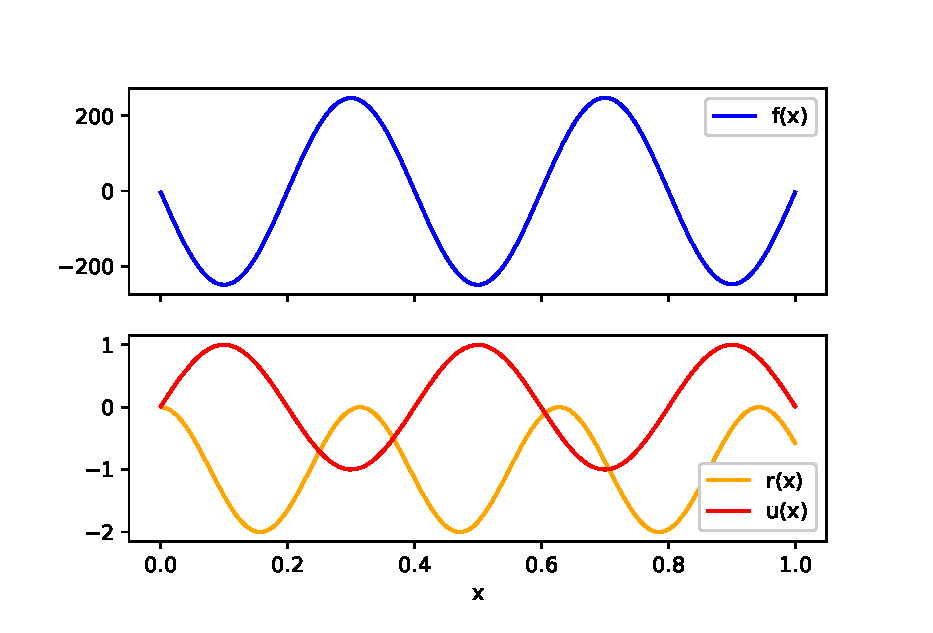
\includegraphics[scale=0.5]{prob_descr}
  \caption{Computation of the exact functions taking place in the ODE.}
  \label{fig:prob_descr}
\end{figure}

Now, in order to solve the problem we have discretized the equation as follos: Given $N>0$ and $h = \frac{1}{N+1}$ amb $x_n = nh$, $0 \leq n \leq N+1$. Then the system reads,

\begin{equation}
\frac{1}{h^2} (u_{n-1}-2u_n+u_{n+1})+r(x_n)u_n = f(x_n), \quad n = 1 ... N
\end{equation}

where $u(x_n) \approx u_n$ and $u_0 = u_{N+1} = 0$. We solved the problem using the following Jacobi iteration,

\begin{equation}
	u_n^{k+1} = \frac{u_{n-1}^k + u_{n+1}^k - h^2 f(x_n)}{2.0 - h^2 r(x_n)}.
\end{equation}

We used 20 processes and converged to the right solution in around 25000 steps as you can see in Figure \ref{fig:MSE_dec}; where after that point the $MSE$ is stable around 0. Furthermore, to see how the Jacobi iteration process gets to the right solution, we provide with a plot of the estimation at different stages (Figure \ref{fig:func_appr}).

The code we used for this computation is presented in Listing \ref{lst:ode_jacobi}. Also, the printing functions are also shown in Listing \ref{lst:printing_jacobi}.

\begin{figure}[H]
  \centering
  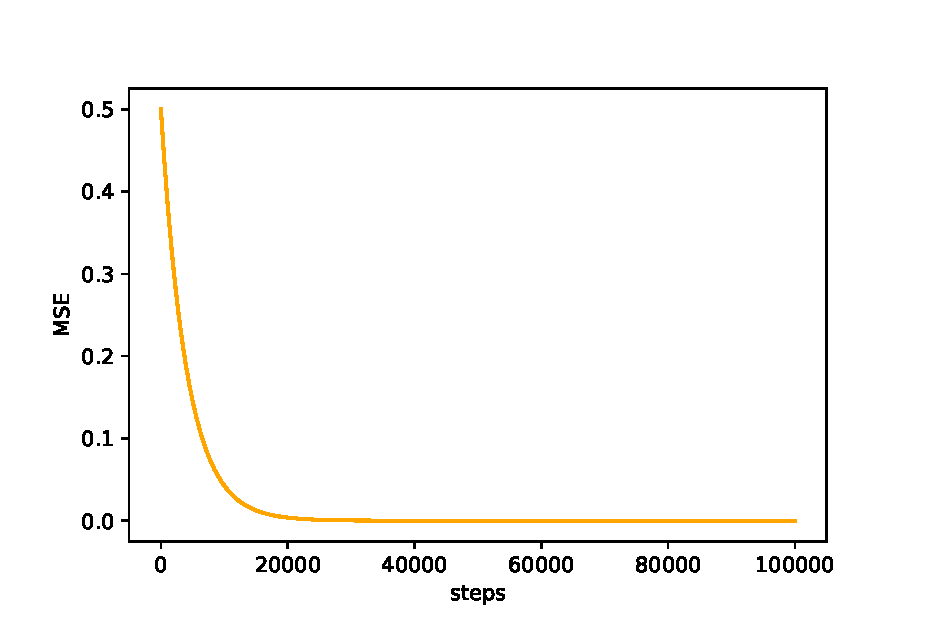
\includegraphics[scale=0.5]{MSE_dec}
  \caption{Decrease of the MSE at each iteration of the Jacobi iteration process.}
  \label{fig:MSE_dec}
\end{figure}

\begin{figure}[H]
  \centering
  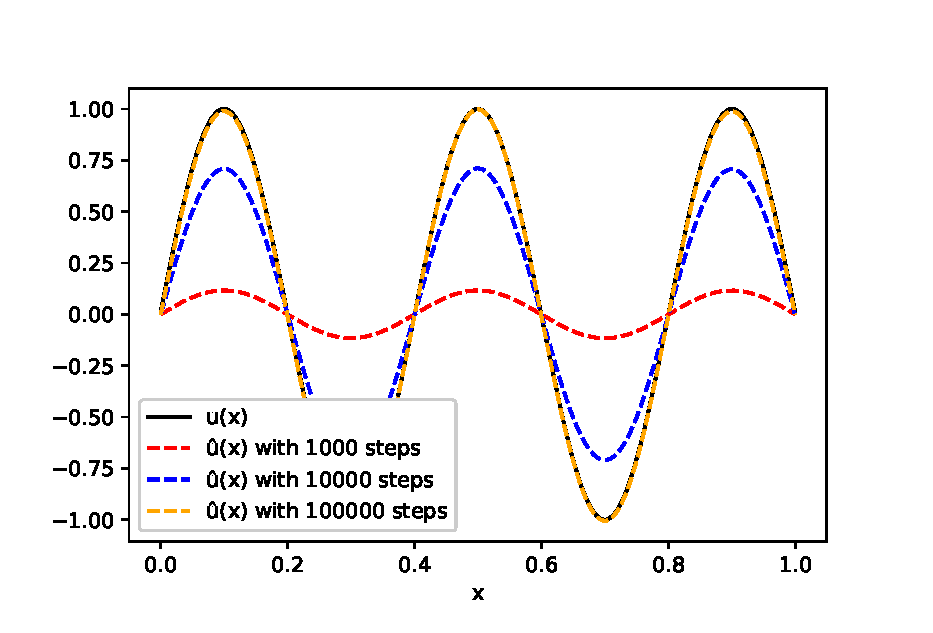
\includegraphics[scale=0.5]{func_appr}
  \caption{Estimation of the $u(x)$ function using the Jacobi iteration process with different number of iterations.}
  \label{fig:func_appr}
\end{figure}

\begin{lstlisting}[style=customc, caption={MPI implementation of an ODE solver using Jacobi iteration process}, label={lst:ode_jacobi}]
#include <stdio.h>
#include <stdlib.h>
#include <math.h>
#include <mpi.h>
#include <string.h>

#define N 1000 // number of inner grid points
#define SMX 1000000 // number of iterations
#define M_PI 3.14159265358979323846 // PI
#define H (1.0 / (N + 1.0)) // The first and last points x = 0, 1 must be 0
#define BLACK 0
#define RED 1

double r_func(double x)
{
  return cos(20*x) - 1.0;
}

double u_func(double x)
{
  return sin(5*M_PI*x);
}

double f_func(double x)
{
  return sin(5*M_PI*x)*(cos(20*x) - 1) - 25*M_PI*M_PI*sin(5*M_PI*x);
}

int main(int argc, char* argv[])
{
  /* Local variables */
  int size, rank, rc, tag;
  MPI_Status status;
  tag = 5;

  /* Initialize MPI */
  rc = MPI_Init(&argc, &argv);
  rc = MPI_Comm_size(MPI_COMM_WORLD, &size);
  rc = MPI_Comm_rank(MPI_COMM_WORLD, &rank);
  if (N < size){
    fprintf(stderr, "%s\n", "Too few discretization points...");
    exit(1);
  }

  /* Linear data distribution */
  int Ip, inVal, M_tild, L, R, a;
  a = 2;
  M_tild = N + (size - 1)*a;
  L = M_tild / size;
  R = M_tild % size;
  Ip = L + (rank < R ? 1: 0);
  inVal = (L-a)*rank + (rank < R ? rank : R);

  /* Create the data */
  double u_real[Ip], u[Ip], u_new[Ip];
  double f[Ip], r[Ip];
  double se;
  double mse[SMX];

  /* Create the x values */
  double x[Ip];
  for (unsigned int i = 0; i < Ip; i++){
    x[i] = (inVal + i + 1)*H;
  }

  /* Compute the real values of u that we are going to use for the error */
  /* Also, compute the values of the functions so we don't need to do calculations
     at each iteration */
  for (unsigned int i = 0; i < Ip; i++){
    u_real[i] = u_func(x[i]);
    f[i] = f_func(x[i]);
    r[i] = r_func(x[i]);
    u[i] = 0.0;
  }

  /* Actual computation */
  for (unsigned int step = 0; step < SMX; step++){
    // Communication
    if (rank % 2 == BLACK){
      if (rank < size - 1){ // Avoid sending to P process
        rc = MPI_Send(&u[Ip-2], 1, MPI_DOUBLE, rank+1, tag, MPI_COMM_WORLD);
        rc = MPI_Recv(&u[Ip-1], 1, MPI_DOUBLE, rank+1, tag, MPI_COMM_WORLD, &status);
      }
      if (rank > 0){ // Avoid sending to -1 process
        rc = MPI_Send(&u[1], 1, MPI_DOUBLE, rank-1, tag, MPI_COMM_WORLD);
        rc = MPI_Recv(&u[0], 1, MPI_DOUBLE, rank-1, tag, MPI_COMM_WORLD, &status);
      }
    } else{ // rank % 2 == RED
      if (rank > 0){ // Avoid sending to -1 process
        rc = MPI_Recv(&u[0], 1, MPI_DOUBLE, rank-1, tag, MPI_COMM_WORLD, &status);
        rc = MPI_Send(&u[1], 1, MPI_DOUBLE, rank-1, tag, MPI_COMM_WORLD);
      }
      if (rank < size - 1){ // Avoid sending to (size) process
        rc = MPI_Recv(&u[Ip-1], 1, MPI_DOUBLE, rank+1, tag, MPI_COMM_WORLD, &status);
        rc = MPI_Send(&u[Ip-2], 1, MPI_DOUBLE, rank+1, tag, MPI_COMM_WORLD);
      }
    }
    // Computation of the values
    for (unsigned int i = 1; i < Ip-1; i++){
      u_new[i] = (u[i-1] + u[i+1] - H*H*f[i]) / (2.0 - H*H*r[i]);
    }

    // We update our values and compute the error
    se = 0;
    for (unsigned int i = 0; i < Ip; i++){
      if (i == 0 && rank != 0) continue; // Only the first process uses the first element
      else if(i == Ip-1 && rank != size-1) continue; // Only the last element computes the last element
      u[i] = u_new[i];
      se += (u[i] - u_real[i])*(u[i] - u_real[i]);
    }
    // We share the squared error and compute the mean
    MPI_Allreduce(&se, &mse[step], 1, MPI_DOUBLE, MPI_SUM, MPI_COMM_WORLD);
    mse[step] /= N;
  }

  // Finally we write the error in a file (only one process should do it)
  if (rank == 0){
    FILE *err_fp;
    err_fp = fopen("Files/err_matr.txt","wb"); // Here the name of your file 
    for (unsigned int step = 0; step < SMX; step++){
      fprintf(err_fp, "%.10f\n", mse[step]);
    }
    fclose(err_fp);
  }

  // Also, we write (size) files for the final u approximation
  FILE *u_fp;
  char pId[5];
  char nameFile[50] = "Files/u_matr_stx_10000_p";
  sprintf(pId, "%d", rank);
  strcat(nameFile,pId);
  strcat(nameFile, ".txt");
  u_fp = fopen(nameFile,"wb"); // Here the name of your file 
  for (unsigned int i = 0; i < Ip; i++){
    if (i == 0 && rank != 0) continue; // Only the first process prints the first element
    else if (i == Ip-1 && rank != size-1) continue; // Only the last element prints the last element
    fprintf(u_fp, "%.10f\n", u[i]);
  }
  fclose(u_fp);

  /* Finish the process */
  MPI_Finalize();
  exit(0);
}
\end{lstlisting}

\begin{lstlisting}[style=custompy, caption={Reading the files and printing}, label={lst:printing_jacobi}]

import numpy as np
import matplotlib.pyplot as plt

# They were precomputed in C
f_m = np.loadtxt("Files/f_matr.txt")
u_m = np.loadtxt("Files/u_matr.txt")
r_m = np.loadtxt("Files/r_matr.txt")
x_m = np.loadtxt("Files/x_matr.txt")

# Plot of the exact functions
fig, (ax1, ax2) = plt.subplots(2,1,sharex = True)
ax1.plot(x_m, f_m, label = "f(x)", color = "blue")
ax2.plot(x_m, r_m, label = "r(x)", color = "orange")
ax2.plot(x_m, u_m, label = "u(x)", color = "red")
ax1.legend()
ax2.legend()
ax2.set_xlabel("x")
plt.savefig("Files/prob_descr.eps", format = "eps")
plt.plot()

# Get the computed error 
e_m = np.loadtxt("Files/err_matr.txt")

# Plot of the error
fig, ax = plt.subplots()
ax.plot(np.arange(len(e_m)), e_m, color = "orange")
ax.set_ylabel("MSE")
ax.set_xlabel("steps")
plt.savefig("Files/MSE_dec.eps", format = "eps")

# Get the estimation of u
u_tild_m_1000 = np.array(())
for i in range(20):
    name = "Files/u_matr_stx_1000_p" + str(i) + ".txt"
    u_tmp = np.loadtxt(name)
    u_tild_m_1000 = np.hstack((u_tild_m_1000, u_tmp))
u_tild_m_10000 = np.array(())
for i in range(20):
    name = "Files/u_matr_stx_10000_p" + str(i) + ".txt"
    u_tmp = np.loadtxt(name)
    u_tild_m_10000 = np.hstack((u_tild_m_10000, u_tmp))
u_tild_m_100000 = np.array(())
for i in range(20):
    name = "Files/u_matr_stx_100000_p" + str(i) + ".txt"
    u_tmp = np.loadtxt(name)
    u_tild_m_100000 = np.hstack((u_tild_m_100000, u_tmp))

# Plot the estimation
fig, ax = plt.subplots()
ax.plot(x_m, u_m, label = "u(x)", color = "black")
ax.plot(x_m, u_tild_m_1000, label = "u^{^}(x) with 1000 steps", 
        color = "red", linestyle = "dashed")
ax.plot(x_m, u_tild_m_10000, label = "u^{^}(x) with 10000 steps", 
        color = "blue", linestyle = "dashed")
ax.plot(x_m, u_tild_m_100000, label = "u^{^}(x) with 100000 steps", 
        color = "orange", linestyle = "dashed")
ax.legend()
ax.set_xlabel("x")
plt.savefig("Files/func_appr.eps", format = "eps")
\end{lstlisting}


\end{enumerate}

\end{document}